\begin{card}
	\frametitle{Übung 1: Einführung}
	\url{http://people.f4.htw-berlin.de/~hebold/htw/pka/exercises/einf\%C3\%BChrung.pdf}
\end{card}

\begin{card}
	Gegeben: $f_1(x) = x^2-2$, $f_2(x) = x-5$, $f_3(x) = e^{x-2}$,  $f_4(x) = ln(x+5)$, $f_5(x) = 5$
	\vfill
	\begin{columns}
		\begin{column}{.5\linewidth}
		Bestimmen Sie die Ausdrücke der folgenden Funktionen:
			\begin{enumerate}[a)]
			\item $f_1 \circ f_2$
			\item $f_1 \circ f_2 \circ f_3$
			\item $(f_1 + f_4) \circ f_2$
			\item $f_3 \circ (f_1 + f_4) \circ f_2$
			\item $f_4 \circ f_4^{-1}$
			\item $ f_4^{-1} \circ f_4$
			\item $f_2 \circ f_3 \circ f_3^{-1} \circ f_2^{-1}$
			\item $f_1 \circ f_5 \circ f_5^{-1} \circ f_1^{-1}$
			\end{enumerate}
		\end{column}
		\begin{column}{.5\linewidth}
		\pause
		Lösung:
			\begin{enumerate}[a)]
			\item $(x-5)^2-2$
			\item $(e^{x-2}-5)^2-2$
			\item $(x-5)^2-2+ln(x)$
			\item $e^{(x-5)^2-2+ln(x)-2}$
			\item $id \text{ (da } f_4^{-1} \text{existiert)}$
			\item $id \text{ (da } f_4^{-1} \text{existiert)}$
			\item $id \text{ (da } f_2^{-1} \text{,} f_3^{-1} \text{existiert)}$
			\item \lightning ($f_5^{-1}$ existiert nicht)
			\end{enumerate}
		\end{column}
	\end{columns}
	\vfill
	Bilden Umkehrfunktion: $y = ln(x+5) \Leftrightarrow e^y = e^{ln(x+5)} \Leftrightarrow e^y = x+5 \Leftrightarrow e^y-5 = x \Rightarrow y = e^x-5$
\end{card}

\begin{card}
	Schreiben Sie in Java jeweils ein Programm, dass die Funktionen
	\begin{enumerate}[a)]
	\item $x+y$
	\item $x*y$
	\item $x^y$
	\end{enumerate}
	als int-Werten rekursiv berechnet
	\hr
	\begin{lstlisting}[language=Java]
public static int add(int x, int y) {
  if (y == 0) { return x; }
  return 1 + add(x, y-1);
}

public static int multiply(int x, int y) {
  if (y == 0) { return 0; }
  return x + multiply(x, y-1);
}

public static int pow(int x, int y) {
  if (y == 0) { return 1; }
  return x * pow(x, y-1);
}
	\end{lstlisting}
\end{card}

\begin{card}
	Schreiben Sie in Java Programme zu Berechnung der Fakultät mit dem Datentyp BigInteger rekursiv und iterativ.
	\hr
	$n! = 1 \cdot 2 \cdot ... \cdot (n-1) \cdot n = n  \cdot  (n-1)!$
	\begin{lstlisting}[language=Java]
	static int fac(int x) { return x == 0 ? 1 : x * fac(x-1); }
  BI = BigInteger
  static BI faci(BI x) {
    BI result = BI.ONE;
    for (BI i = BI.ONE; i.compareTo(x) <= 0; i = i.add(BI.ONE)) {
      result = result.multiply(i);
    }
    return result;
  }

  static BI facer(BI x) {
    if (x.compareTo(BI.ONE) <= 0) {
        return BI.ONE;
    }
    return x.multiply(facer(x.subtract(BI.ONE)));
  }
	\end{lstlisting}
\end{card}

\begin{card}
	Collatz-Problem Definition:\\
	$f: \mathbb{N} \rightarrow \mathbb{N}$ mit
	$f(1) = 1$, n gerade: $f(n) = n / 2$,n ungerade: $f(n) = 3n + 1$\\
	$F: \mathbb{N} \rightarrow \mathbb{N}$ mit $F(1) = f(1)  = 1$, $F(n) = F(f(n))$

	Collatz-Problem: Ist F für jedes $n \in \mathbb{N}$  definiert, d.h. $\forall n \in \mathbb{N}$ $\exists$ $F(n) \in \mathbb{N}$?
	\hr
	\begin{lstlisting}[language=Java]
static int f(int x) {
  if (x == 1) { return 1; }
  else if (x % 2 == 0) { return x / 2; }
  return 3 * x + 1;
}
static int F(int x) {
  if (x == 1) return 1;
  System.out.print("[" + x + "]");
  return F(f(x));
}
static int Flength(int x, int c) {
  if (x == 1) return c;
  return Flength(f(x), c + 1);
}
static int Flength(int x) {return Flength(x, 1);}
	\end{lstlisting}
\end{card}

\begin{card}
	Relationen, mit $R \subseteq M \times M$\\
	\begin{tabular}{ll}
		Reflexivität:& $(x, x) \in R $\\
		Symmetrie:&	$(x, y) \in R \Rightarrow (y, x) \in R$\\
		Antisymmetrie:& $(x, y) \in R, (y, x) \in R \Rightarrow x=y$\\
		Asymmetrie:& $(x, y) \in R \Rightarrow (y, x) \notin R$\\
		Transitivität:& $(x, y) \in R, (y, z) \in R \Rightarrow (x, z) \in R$\\
		Funktion: & bijektiv = surjektiv (rechtstotal, isOnto) +\\
	     	      & injektiv (linkseindeutig, isOneOne)
		\end{tabular}
		\begin{figure}[h]
		\centering
		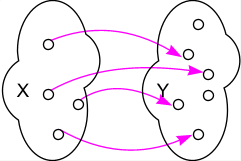
\includegraphics[width=3cm]{Injektivitaet_Mengenwolke}
		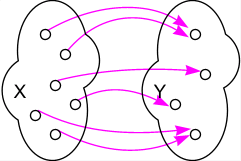
\includegraphics[width=3cm]{Surjektivitaet_Mengenwolke}
		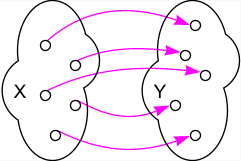
\includegraphics[width=3cm]{Bijektivitaet_Mengenwolke}
		\caption{injektive, surjektive, bijektive Abbildung}
		\end{figure}
\end{card}

\begin{card}
	Mengen: $A = \{3, 4\}$, $B = \{\{3, 4\}\}$\\Welche Behauptung stimmt?
	\begin{enumerate}[a)]
	\item $A = B$
	\item $A \subseteq B$
	\item $A \subsetneq B$
	\item $|A| = |B|$
	\end{enumerate}
	\hr
	\begin{enumerate}[a)]
	\item Nein, da unterschiedlich mächtig. siehe 4.)
	\item Nein, da gelten muss: $\forall x \in A: x \in B$, aber hier: $3,4 \notin B$
	\item A keine echte Teilmenge von B, da gelten muss: $A \subset B \land A \neq B \Rightarrow a.) \land \lnot b.)$ , a.) ist falsch
	\item Nein, da $2 \neq 1$
	\end{enumerate}
\end{card}

\begin{card}
	Das kartesische Produkt zweier Mengen A und B ist wie folgt definiert:
	$A \times B = \{(x,y):x	\in	A \land	y \in B\}$\\
	Prüfen Sie, ob das kartesische Produkt assoziativ ist, d.h. ob für Mengen X,Y,Z gilt:
	$(X	\times Y)\times Z=X \times(Y \times Z)$
	\hr
	Nein, da die Tupel $((x,y),z)$ und $(x,(y,z))$ unterschiedlich sind, also eine andere Struktur haben.
\end{card}

\begin{card}
	Welcher der folgenden Ausdrücke ist korrekt?
	\begin{enumerate}[a)]
	\item $0 \in \emptyset$
	\item $0 = \emptyset$
	\item $0 \subseteq \emptyset$
	\item $\{0\} \subseteq \emptyset$
	\end{enumerate}
	\hr
	\begin{enumerate}[a)]
	\item Nein, die leere Menge hat keine Elemente
	\item Nein, Zahlen sind keine Menge
	\item Nein, siehe b.)
	\item Nein, siehe a.)
	\end{enumerate}
\end{card}

\begin{card}
	Sei X eine Menge endlicher Größe und $2^X$ die Potenzmenge von $X$. Welches Ergebnis liefern:
	\begin{enumerate}[a)]
	\item $|2^X \cup X|$
	\item $|2^X| \cup |X|$
	\end{enumerate}
	\hr
	Beispiel: Potenzmenge  $X = \{ a,b \} \Rightarrow 2^X = \{ \emptyset, \{ a \}, \{ b \} , \{ a,b \} \}$
	\begin{enumerate}[a)]
	\item $2^X \cup X = \{ \emptyset, \{ a \}, \{ b \} , \{ a,b \}, a, b\} \Rightarrow
	|2^X \cup X| = 2^{|X|} + |X|$
	\item \lightning Vereinigung ist nur auf Mengen definiert und nicht auf Zahlen.
	\end{enumerate}
\end{card}
